\documentclass[handout, 11pt]{beamer}
\mode
<presentation>{\usetheme{Madrid}}
\institute[UF]{\inst{1}
University of Florida\\
Department of Finance, Insurance, and Real Estate}
\usepackage{xcolor}
\setbeamertemplate{headline}{\begin{beamercolorbox}[ht=2.25ex, dp=3.75ex]{section in head/foot}
\insertnavigation{\paperwidth}
\end{beamercolorbox}}
\AtBeginSection{\begin{frame}
\frametitle{Table of Contents}
\tableofcontents[currentsection]
\end{frame}}
\begin{document}
\title[Modeling Road-map]{Advanced Financial Modeling}
\subtitle{A Road-map to Learning Advanced Financial Modeling Topics}
\author[DeRobertis]{Nick DeRobertis\inst{1}}
\date{\today}
\begin{frame}
\titlepage
\label{title-frame}
\end{frame}
\begin{section}{Introduction}
\begin{frame}
\frametitle{What we Covered and What is Left}
\begin{itemize}
\small
\vfill
\item Throughout the Financial Modeling with Python and Excel course, we have covered Python and Excel basics
\vfill
\item We have also covered financial modeling specifics, such as how to structure a financial model in both Python and Excel, cash flow and probability modeling, sensitivity analysis, scenario analysis, and Monte Carlo simulations
\vfill
\item As far as types of financial models, we covered a retirement model, a capital budgeting model, a lender profitability model, and the discounted cash flow (DCF) valuation of a stock
\vfill
\item There is a lot I didn't cover in that course. Let's do a quick overview of it today.
\vfill
\item This will serve as a roadmap to learn additional topics after completing the first course. This is also the beginning of a new Advanced Financial Modeling with Python course
\end{itemize}
\end{frame}
\end{section}
\begin{section}{Types of Financial Models}
\begin{frame}
\frametitle{Financial Models 1}
\begin{itemize}
\item \underline{Portfolio valuation and optimization}: Find the returns, value, and risk of a portfolio and select the best asset allocation for the portfolio
\vfill
\item \underline{Additional Funds Needed (AFN)}: Budgeting model which uses forecasted financial statements to determine how much capital should be raised
\vfill
\item \underline{Lease or Own}: Guides the decision of whether to rent or buy an asset
\vfill
\item \underline{Event Studies}: Tries to determine the impact of an event
\vfill
\item \underline{Merger and Aquisition (M\&A)}: A DCF valuation of a target company with operations being combined with the parent at a merger date. Detetermines M\&A price.
\end{itemize}
\end{frame}
\begin{frame}
\frametitle{Financial Models 2}
\begin{itemize}
\item \underline{Leveraged Buyout (LBO)}: A specialized M\&A model used for when large amounts of debt are being used to purchase the target firm.
\vfill
\item \underline{Derivatives Valuation}: Value options, swaps, forwards, etc.
\vfill
\item \underline{Debt models}: Immunization models are about having the right amount of cash in the future, term structure models estimate the rates for different maturity bonds, and default-adjusted return models factor in default in determining debt returns
\vfill
\item \underline{Value at Risk (VaR)}: Determine how much an investment might lose with a certain probability in a certain time span
\end{itemize}
\end{frame}
\begin{frame}
\frametitle{Financial Model Resources}
\begin{itemize}
\item Here are some links with free resources to learn more about types of models
\vfill
\item The following examples will be using Excel only
\vfill
\item \textcolor{blue}{\underline{\href{http://macabacus.com/learn}{Macabacus}}}
\vfill
\item \textcolor{blue}{\underline{\href{https://corporatefinanceinstitute.com/resources/knowledge/modeling/}{Corporate Finance Institute}}}
\vfill
\item \textcolor{blue}{\underline{\href{https://fminstitute.com/learning/}{Financial Modeling Institute}}}
\vfill
\item And I found a couple Python resources, though the coding standards are not great:
\vfill
\item \textcolor{blue}{\underline{\href{http://www.financeandpython.com/Finance.html}{Finance and Python}}}
\vfill
\item \textcolor{blue}{\underline{\href{https://www.datacamp.com/community/tutorials/finance-python-trading}{Build a Trading Algorithm in Python}}}
\end{itemize}
\end{frame}
\end{section}
\begin{section}{Data Pipelines}
\begin{frame}
\begin{columns}
\begin{column}{0.5\textwidth}
\vbox to 0.8\textheight{\begin{itemize}
\item Data pipelines are about getting the input data into your model in a standardized way
\vfill
\item Within data pipelines, there are two main steps: data collection and data wrangling (cleaning + reformatting).
\vfill
\item Either step can be automated, ideally both would be, but it always comes down to a tradeoff with modeler time
\end{itemize}}
\end{column}
\begin{column}{0.5\textwidth}
\vbox to 0.8\textheight{\centering
\vfill
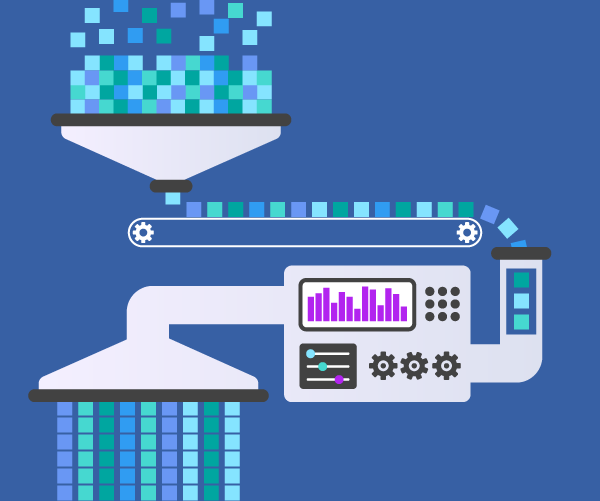
\includegraphics[height=1.0\textheight, keepaspectratio, width=0.9\textwidth]{Sources/data-pipeline.png}
\vfill
\vfill}
\end{column}
\end{columns}
\end{frame}
\begin{frame}
\frametitle{Data Collection}
\begin{itemize}
\small
\vfill
\item Data can come from many sources, but most typically it originates from the Internet
\vfill
\item If you can manually download the data, you can automate it via web scraping
\vfill
\item You can also extract different types of data with web scraping, even if it is not structured as a dataset
\vfill
\item Some data comes from an API, where you need to send requests to download the data
\vfill
\item \texttt{selenium}
uses Python code to drive a browser such as Chrome while
\texttt{requests}
is a more lightweight, text based way to make web requests (good for APIs).
\vfill
\item Another common source of data is SQL databases. While you will still need to have a basic understanding of SQL to query them, Python can help with
\texttt{SQLAlchemy}
which allows
you to write the queries in Python.
\texttt{pandas}
also has functionality to work with SQL
\end{itemize}
\end{frame}
\begin{frame}
\frametitle{Data Wrangling}
\begin{itemize}
\small
\vfill
\item We have already covered the best general-purpose tool for wrangling data:
\texttt{pandas}
\vfill
\item We did not cover it in enough detail to cover all data cleaning cases
\vfill
\item The main material left is selecting, merging, grouping, and reshaping
\vfill
\item Even if your data is without issues, you may still need to change the format, combine sources, aggregate, etc.
\vfill
\item Regular expressions are a way of matching any possible string and extracting parts of it, which useful for messy data
\end{itemize}
\end{frame}
\begin{frame}
\frametitle{Data Pipelines Resources}
\begin{itemize}
\item \textcolor{blue}{\underline{\href{https://stackabuse.com/getting-started-with-selenium-and-python/}{Get Started Browser-Based Web Scraping with Selenium}}}
\vfill
\item \textcolor{blue}{\underline{\href{https://github.com/mherrmann/selenium-python-helium}{Helium - A Higher-Level API to Selenium}}}
\vfill
\item \textcolor{blue}{\underline{\href{https://realpython.com/python-requests/}{Get Started Text-Based Web Scraping with Requests}}}
\vfill
\item \textcolor{blue}{\underline{\href{https://pandas.pydata.org/pandas-docs/stable/getting\_started/10min.html}{Pandas Intro, Covers Basics of Needed Topics}}}
\vfill
\item \textcolor{blue}{\underline{\href{https://pandas.pydata.org/pandas-docs/stable/user\_guide/cookbook.html\#cookbook}{Advanced Pandas}}}
\vfill
\item \textcolor{blue}{\underline{\href{https://scotch.io/tutorials/an-introduction-to-regex-in-python}{Intro to Regular Expressions}}}
\vfill
\item \textcolor{blue}{\underline{\href{https://docs.python.org/3/library/re.html}{Regular Expression Reference}}}
\vfill
\item \textcolor{blue}{\underline{\href{https://auth0.com/blog/sqlalchemy-orm-tutorial-for-python-developers/}{SQLAlchemy Overview Tutorial}}}
\vfill
\item \textcolor{blue}{\underline{\href{https://towardsdatascience.com/sqlalchemy-python-tutorial-79a577141a91}{SQLAlchemy Simple Tutorial and Examples}}}
\vfill
\item \textcolor{blue}{\underline{\href{https://docs.sqlalchemy.org/en/13/intro.html}{SQLAlchemy Documentation}}}
\end{itemize}
\end{frame}
\end{section}
\begin{section}{Mathematical Tools}
\begin{frame}
\frametitle{What Math we Covered}
\begin{columns}
\begin{column}{0.5\textwidth}
\vbox to 0.8\textheight{\begin{itemize}
\item We covered basic mathematical tools including basic probability theory, algebra, variance/standard deviation, averages, and basic regressions
\vfill
\item Most financial modeling does not take very advanced math, with the exception of some derivatives models
\vfill
\item But there are a few more useful tools we didn't have time to cover
\end{itemize}}
\end{column}
\begin{column}{0.5\textwidth}
\vbox to 0.8\textheight{\centering
\vfill

\includegraphics[height=1.0\textheight, keepaspectratio, width=0.9\textwidth]{Sources/equations-chalkboard-2.jpg}
\vfill
\vfill}
\end{column}
\end{columns}
\end{frame}
\begin{frame}
\frametitle{General Math Tools}
\begin{itemize}
\item Often we want to maximize or minimize something, e.g. maximize returns or NPV, minimize risk. We can do this in general with a mathematical technique called
\underline{optimization}
\vfill
\item If you have a complicated custom model, such that the algebra is getting too difficult to do by hand, you can use a
\underline{computer algebra system}
\vfill
\item \underline{Levenshtein (edit) distance}
can be used to say how similar two strings are,
which is useful for data cleaning and more.
\end{itemize}
\end{frame}
\begin{frame}
\frametitle{Statistics Tools}
\begin{itemize}
\item We covered Ordinary Least Squares (OLS) regressions, which is what anyone means if they just say regression
\vfill
\item There are many more kinds of regressions, we can't even mention them all here. But most likely to be useful include
\underline{logistic regression}
for when
probabilities are dependent variables and
\underline{panel regression + fixed effects}
for when you are dealing
with multiple instruments over time
\vfill
\item There are many time-series models to cover, as was mentioned in the forecasting lecture
\vfill
\item \underline{Machine learning/AI}
can be used to make classifications or predictions
\end{itemize}
\end{frame}
\begin{frame}
\frametitle{Mathematical Tools Resources}
\begin{itemize}
\item \textcolor{blue}{\underline{\href{https://towardsdatascience.com/optimization-with-scipy-and-application-ideas-to-machine-learning-81d39c7938b8}{Optimization with SciPy}}}
\vfill
\item \textcolor{blue}{\underline{\href{https://docs.sympy.org/latest/tutorial/preliminaries.html}{Computer Algebra with SymPy}}}
\vfill
\item \textcolor{blue}{\underline{\href{https://www.geeksforgeeks.org/fuzzywuzzy-python-library/}{Levenshtein Distance using fuzzywuzzy}}}
\vfill
\item \textcolor{blue}{\underline{\href{https://towardsdatascience.com/logistic-regression-python-7c451928efee}{Intro to Logistic Regression in Python}}}
\vfill
\item \textcolor{blue}{\underline{\href{https://medium.com/pew-research-center-decoded/using-fixed-and-random-effects-models-for-panel-data-in-python-a795865736ab}{Intro to Panel Regression in Python}}}
\vfill
\item \textcolor{blue}{\underline{\href{https://www.statsmodels.org/stable/py-modindex.html}{Statistical Models in statsmodels}}}
\vfill
\item \textcolor{blue}{\underline{\href{https://bashtage.github.io/linearmodels/doc/index.html}{More Statistical Models in linearmodels}}}
\vfill
\item \textcolor{blue}{\underline{\href{https://docs.scipy.org/doc/scipy/reference/stats.html}{More Statistical Tools in Scipy}}}
\vfill
\item \textcolor{blue}{\underline{\href{https://machinelearningmastery.com/machine-learning-in-python-step-by-step/}{Getting Started with Machine Learning in Python}}}
\vfill
\item \textcolor{blue}{\underline{\href{https://machinelearningmastery.com/start-here/}{General Introduction to Machine Learning}}}
\vfill
\item \textcolor{blue}{\underline{\href{https://datacamp.com/community/tutorials/deep-learning-python}{Deep Learning (AI) in Python using Keras}}}
\vfill
\item \textcolor{blue}{\underline{\href{https://github.com/automl/auto-sklearn/}{Automated Machine Learning with auto-sklearn}}}
\end{itemize}
\end{frame}
\end{section}
\begin{section}{Present Results}
\begin{frame}
\frametitle{Presenting Model Results}
\begin{columns}
\begin{column}{0.5\textwidth}
\vbox to 0.8\textheight{\begin{itemize}
\item We didn't have very much time to cover presenting the model in Python, other than formatting text
\vfill
\item For Excel, the model is already presented so just structure the workbook well
\vfill
\item A well structured Jupyter notebook or Python script is important for another modeler to pick up where you left off. But it still is not an ideal format for non-technical consumers of your model
\end{itemize}}
\end{column}
\begin{column}{0.5\textwidth}
\vbox to 0.8\textheight{\centering
\vfill
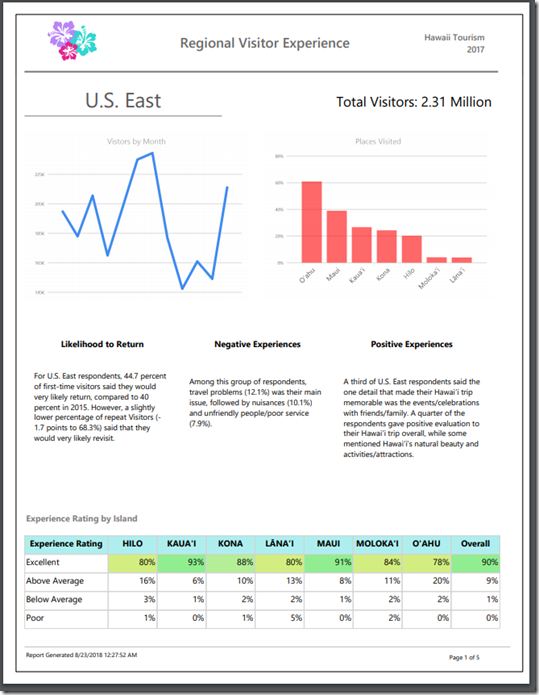
\includegraphics[height=1.0\textheight, keepaspectratio, width=0.9\textwidth]{Sources/example-report.png}
\vfill
\vfill}
\end{column}
\end{columns}
\end{frame}
\begin{frame}
\frametitle{Present with Basic Jupyter}
\begin{itemize}
\item One easy way that doesn't require anything we haven't learned is separating model logic and presentation
\vfill
\item Develop as you will while building the model. But when it's time to share the results, separate the main model logic (classes and functions) into separate Python file(s)
\vfill
\item Then the Jupyter notebook will just show high-level calls to your model and the results
\end{itemize}
\end{frame}
\begin{frame}
\frametitle{Create Reports}
\begin{itemize}
\item Less technical consumers of the model may just want the model conclusions and not to actually use the model themselves
\vfill
\item In this case, it is useful to generate reports containing the model results
\vfill
\item There are three major ways to make reports: HTML, LaTeX, and direct PDF solutions
\vfill
\item If all you need is PDF output, a direct solution is fine, but HTML and LaTeX (which can be converted to HTML) can both be converted to PDF and have the added advantage of being viewable as a web page
\vfill
\item Templating is also easier with HTML and LaTeX
\end{itemize}
\end{frame}
\begin{frame}
\frametitle{Publish Reports and Models}
\begin{itemize}
\item There is another way for non-technical consumers of your model to interact with it: via an app
\vfill
\item It is possible to build apps right in a Jupyter notebook using widgets
\vfill
\item A web app could also be created with a web framework
\vfill
\item With an app, a non-technical consumer of your model can adjust the inputs and see the outputs, without having any knowledge of Python or instructions
\end{itemize}
\end{frame}
\begin{frame}
\frametitle{Advanced Plotting}
\begin{itemize}
\item We covered very basic plots using
\texttt{pandas}
\vfill
\item \texttt{matplotlib}
provides all the plotting functionality to
\texttt{pandas}
and any
\texttt{pandas}
plots can be adjusted using
\texttt{matplotlib}
options
\vfill
\item Several libraries exist for interactive plots, which allow for dropdowns, sliders, selecting points, zooming, tooltips, and more
\vfill
\item Other plotting styles are becoming more popular, such as
\texttt{holoviews},
in which
you just describe the data and it can generate interactive plots for you
\end{itemize}
\end{frame}
\begin{frame}
\frametitle{Presentation Resources}
\begin{itemize}
\small
\vfill
\item \textcolor{blue}{\underline{\href{https://dev.to/goyder/automatic-reporting-in-python---part-1-from-planning-to-hello-world-32n1}{Intro to Creating HTML Reports in Python}}}
\vfill
\item \textcolor{blue}{\underline{\href{https://towardsdatascience.com/creating-pdf-reports-with-python-pdfkit-and-jinja2-templates-64a89158fa2d}{Create HTML Reports and Output to PDF}}}
\vfill
\item \textcolor{blue}{\underline{\href{https://realpython.com/primer-on-jinja-templating/}{Templating HTML and LaTeX Using Jinja}}}
\vfill
\item \textcolor{blue}{\underline{\href{https://www.reportlab.com/docs/reportlab-userguide.pdf}{Direct PDF Output with Reportlab}}}
\vfill
\item \textcolor{blue}{\underline{\href{https://nickderobertis.github.io/py-ex-latex/}{Direct to LaTeX Using pyexlatex}}}
\vfill
\item \textcolor{blue}{\underline{\href{https://www.datacamp.com/community/tutorials/matplotlib-tutorial-python}{Matplotlib Plotting Tutorial}}}
\vfill
\item \textcolor{blue}{\underline{\href{https://holoviews.org/getting\_started/index.html}{Get started with Holoviews}}}
\vfill
\item \textcolor{blue}{\underline{\href{https://www.youtube.com/watch?v=L91rd1D6XTA\&ab\_channel=Enthought}{Introduction to Panel for Building Apps in Jupyter}}}
\vfill
\item \textcolor{blue}{\underline{\href{https://panel.holoviz.org/getting\_started/index.html}{Tutorial for Panel}}}
\vfill
\item \textcolor{blue}{\underline{\href{https://voila.readthedocs.io/en/stable/}{Convert a Jupyter Notebook to a Web App using Voila}}}
\vfill
\item \textcolor{blue}{\underline{\href{https://voila-gallery.org/services/gallery/}{Examples of Voila Web Apps}}}
\vfill
\item \textcolor{blue}{\underline{\href{https://scotch.io/tutorials/getting-started-with-flask-a-python-microframework}{Get Started Building Web Apps with Flask}}}
\vfill
\item \textcolor{blue}{\underline{\href{https://anvil.works/learn/tutorials/jupyter-notebook-to-web-app}{Convert a Jupyter Notebook to a Web App using Anvil}}}
\vfill
\item \textcolor{blue}{\underline{\href{https://www.fullstackpython.com/}{Full Tutorials for Python Web Development}}}
\end{itemize}
\end{frame}
\end{section}
\begin{section}{Programming}
\begin{frame}
\frametitle{Your Programming Future}
\begin{columns}
\begin{column}{0.5\textwidth}
\vbox to 0.8\textheight{\begin{itemize}
\item We were only able to cover basic Python, and certainly not a lot of practices that would typically be used in programming
\vfill
\item Python is very flexible in that you can be productive in it with very little understanding or mastery of it
\vfill
\item But if you do gain a greater knowledge of it, it can unlock new potential.
\vfill
\item Further, there is more we can learn from the software engineering world in how to improve our programming
\end{itemize}}
\end{column}
\begin{column}{0.5\textwidth}
\vbox to 0.8\textheight{\centering
\vfill
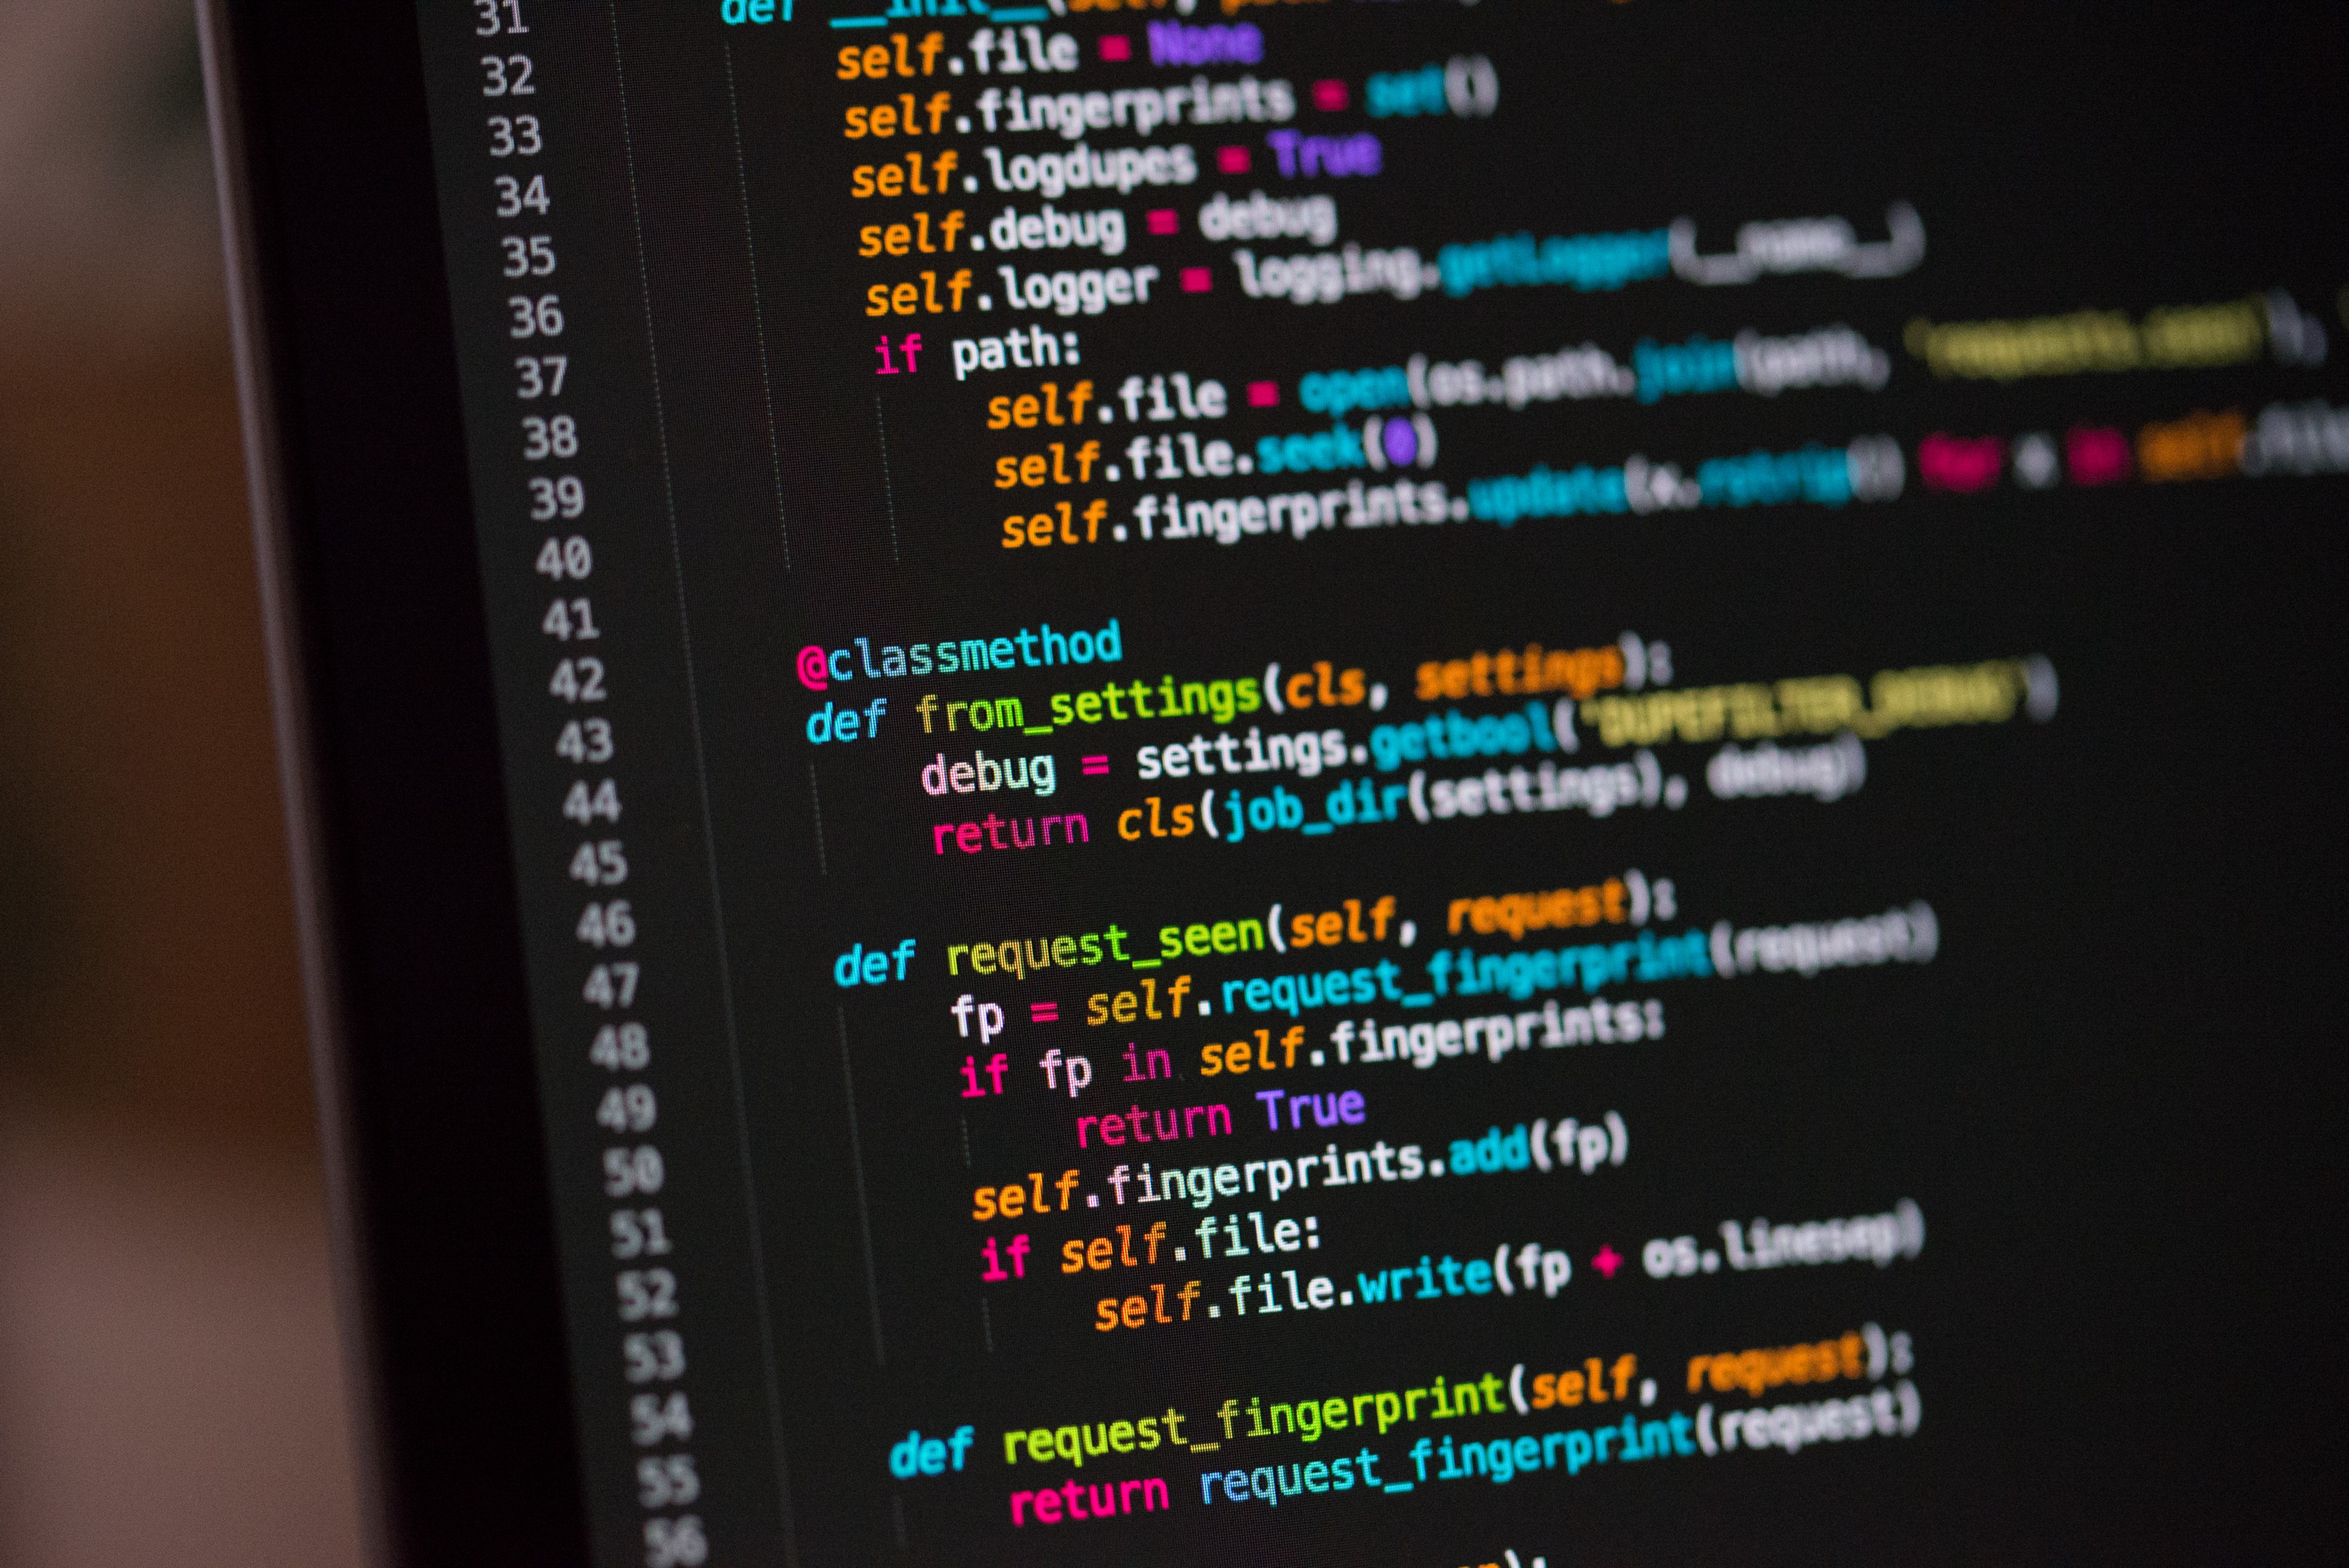
\includegraphics[height=1.0\textheight, keepaspectratio, width=0.9\textwidth]{Sources/python-code-blur.jpeg}
\vfill
\vfill}
\end{column}
\end{columns}
\end{frame}
\begin{frame}
\frametitle{General Programming}
\begin{itemize}
\small
\vfill
\item We can learn a few things from the software engineers that are programming all day every day
\vfill
\item \underline{Version control}
or
\underline{source control}
is a way of tracking
changes to code over time. You can get the full history of the project, and multiple
people can work on the same project at the same time and later merge the changes together.
\texttt{git}
is the gold standard for this.
\vfill
\item Share
\texttt{git}
repositories with the world via Github (or others), allowing anyone to use and improve your project
\vfill
\item Automated testing of your code allows you to make changes ensuring it won't break anything
\vfill
\item Input validation is useful for when others interact with your model directly
\vfill
\item Use an integrated development environment (IDE) such as PyCharm or VS Code for better code completion and linking
\vfill
\item Automatically run tests, style your code, deploy Python packages or web apps, and more with continuous integration/continuous deployment (CI/CD)
\end{itemize}
\end{frame}
\begin{frame}
\frametitle{Python Programming}
\begin{itemize}
\item Python can work with the files on your computer through the
\texttt{open}
command and the
\texttt{os}
\texttt{pathlib}
and
\texttt{shutil}
modules
\vfill
\item Get unique items, unions, intersections using sets
\vfill
\item Override how objects work by overriding double-underscore (dunder) class methods
\vfill
\item Modify existing functions using decorators
\vfill
\item Store Python objects by pickling them
\vfill
\item Check yourself, make your code easier to understand, and power up your IDE using type annotations
\vfill
\item Structure projects using packages and modules
\vfill
\item Isolate project requirements using virtual environments
\end{itemize}
\end{frame}
\begin{frame}
\frametitle{Programming Resources 1}
\begin{itemize}
\small
\vfill
\item \textcolor{blue}{\underline{\href{https://product.hubspot.com/blog/git-and-github-tutorial-for-beginners}{Get Started with Git and Github}}}
\vfill
\item \textcolor{blue}{\underline{\href{https://desktop.github.com/}{Github Desktop is an App that Makes Git Easy}}}
\vfill
\item \textcolor{blue}{\underline{\href{https://realpython.com/python-testing/}{Get Started with Automated Testing in Python}}}
\vfill
\item \textcolor{blue}{\underline{\href{https://www.youtube.com/watch?v=IL3eZYiV70g}{Intro to Input Validation in Python}}}
\vfill
\item \textcolor{blue}{\underline{\href{https://www.jetbrains.com/pycharm/}{PyCharm IDE}}}
\vfill
\item \textcolor{blue}{\underline{\href{https://code.visualstudio.com/}{Visual Studio Code (VS Code) IDE}}}
\vfill
\item \textcolor{blue}{\underline{\href{https://semaphoreci.com/blog/cicd-pipeline}{Intro to CI/CD}}}
\vfill
\item \textcolor{blue}{\underline{\href{https://github.com/features/actions}{CI/CD Using Github Actions}}}
\vfill
\item \textcolor{blue}{\underline{\href{https://www.pythonforbeginners.com/files/reading-and-writing-files-in-python}{Intro to Reading and Writing Files with Python}}}
\vfill
\item \textcolor{blue}{\underline{\href{https://realpython.com/python-pathlib/}{Beyond the Basics of Working with Files in Python}}}
\end{itemize}
\end{frame}
\begin{frame}
\frametitle{Programming Resources 2}
\begin{itemize}
\small
\vfill
\item \textcolor{blue}{\underline{\href{https://realpython.com/python-sets/}{Work with Sets in Python}}}
\vfill
\item \textcolor{blue}{\underline{\href{https://dbader.org/blog/python-dunder-methods}{Get Started with Dunder Methods in Python}}}
\vfill
\item \textcolor{blue}{\underline{\href{https://realpython.com/python-data-classes/}{Advanced Dataclasses}}}
\vfill
\item \textcolor{blue}{\underline{\href{https://ipython.readthedocs.io/en/stable/config/integrating.html}{Rich Object Display in Jupyter}}}
\vfill
\item \textcolor{blue}{\underline{\href{https://realpython.com/primer-on-python-decorators/}{Get Started with Python Decorators}}}
\vfill
\item \textcolor{blue}{\underline{\href{https://www.datacamp.com/community/tutorials/pickle-python-tutorial}{Store Python Objects with pickle and dill}}}
\vfill
\item \textcolor{blue}{\underline{\href{https://dev.to/dstarner/using-pythons-type-annotations-4cfe}{Intro to Type Annotations in Python}}}
\vfill
\item \textcolor{blue}{\underline{\href{https://docs.python-guide.org/writing/structure/}{Intro to Project Structure in Python}}}
\vfill
\item \textcolor{blue}{\underline{\href{https://www.dabapps.com/blog/introduction-to-pip-and-virtualenv-python/}{Introduction to Virtual Environments in Python}}}
\vfill
\item \textcolor{blue}{\underline{\href{https://realpython.com/pipenv-guide/}{Virtual Environments Made Easy with pipenv}}}
\end{itemize}
\end{frame}
\end{section}
\begin{section}{Extras}
\begin{frame}
\frametitle{General Resources}
\begin{itemize}
\item \textcolor{blue}{\underline{\href{https://docs.python-guide.org/}{The Hitchhiker's Guide to Python}}}
\vfill
\item \textcolor{blue}{\underline{\href{https://realpython.com/}{Real Python}}}
\vfill
\item \textcolor{blue}{\underline{\href{https://automatetheboringstuff.com/}{Automate the Boring Stuff with Python}}}
\vfill
\item \textcolor{blue}{\underline{\href{https://pbpython.com/}{Practical Business Python}}}
\end{itemize}
\end{frame}
\end{section}
\appendix
\newcounter{finalframe}
\setcounter{finalframe}{\value{framenumber}}
\begin{frame}
\frametitle{Lecture Resources}
{
\setbeamercolor{block title}{bg=teal}
\begin{block}{Lecture Resources}
\begin{enumerate}
\item \textcolor{blue}{\underline{\href{https://nickderobertis.github.io/fin-model-course/\_static/generated/pdfs/SA1 Advanced Financial Modeling.pdf}{Slides - Advanced Financial Modeling}}}
\item \textcolor{blue}{\underline{\href{https://nickderobertis.github.io/fin-model-course/\_static/generated/pdfs/LNA1 Advanced Financial Modeling.pdf}{Lecture Notes - Advanced Financial Modeling}}}
\end{enumerate}
\vfill
\end{block}
}
\label{frames:resources}
\end{frame}
\setcounter{framenumber}{\value{finalframe}}
\end{document}